\begin{enumerate}
	\item Exercício
	
	\begin{figure}[htb]
		\caption{Integrais duplas - Aula 8 - Exercício I}
		\label{v08_a08_e01}
		\centering
		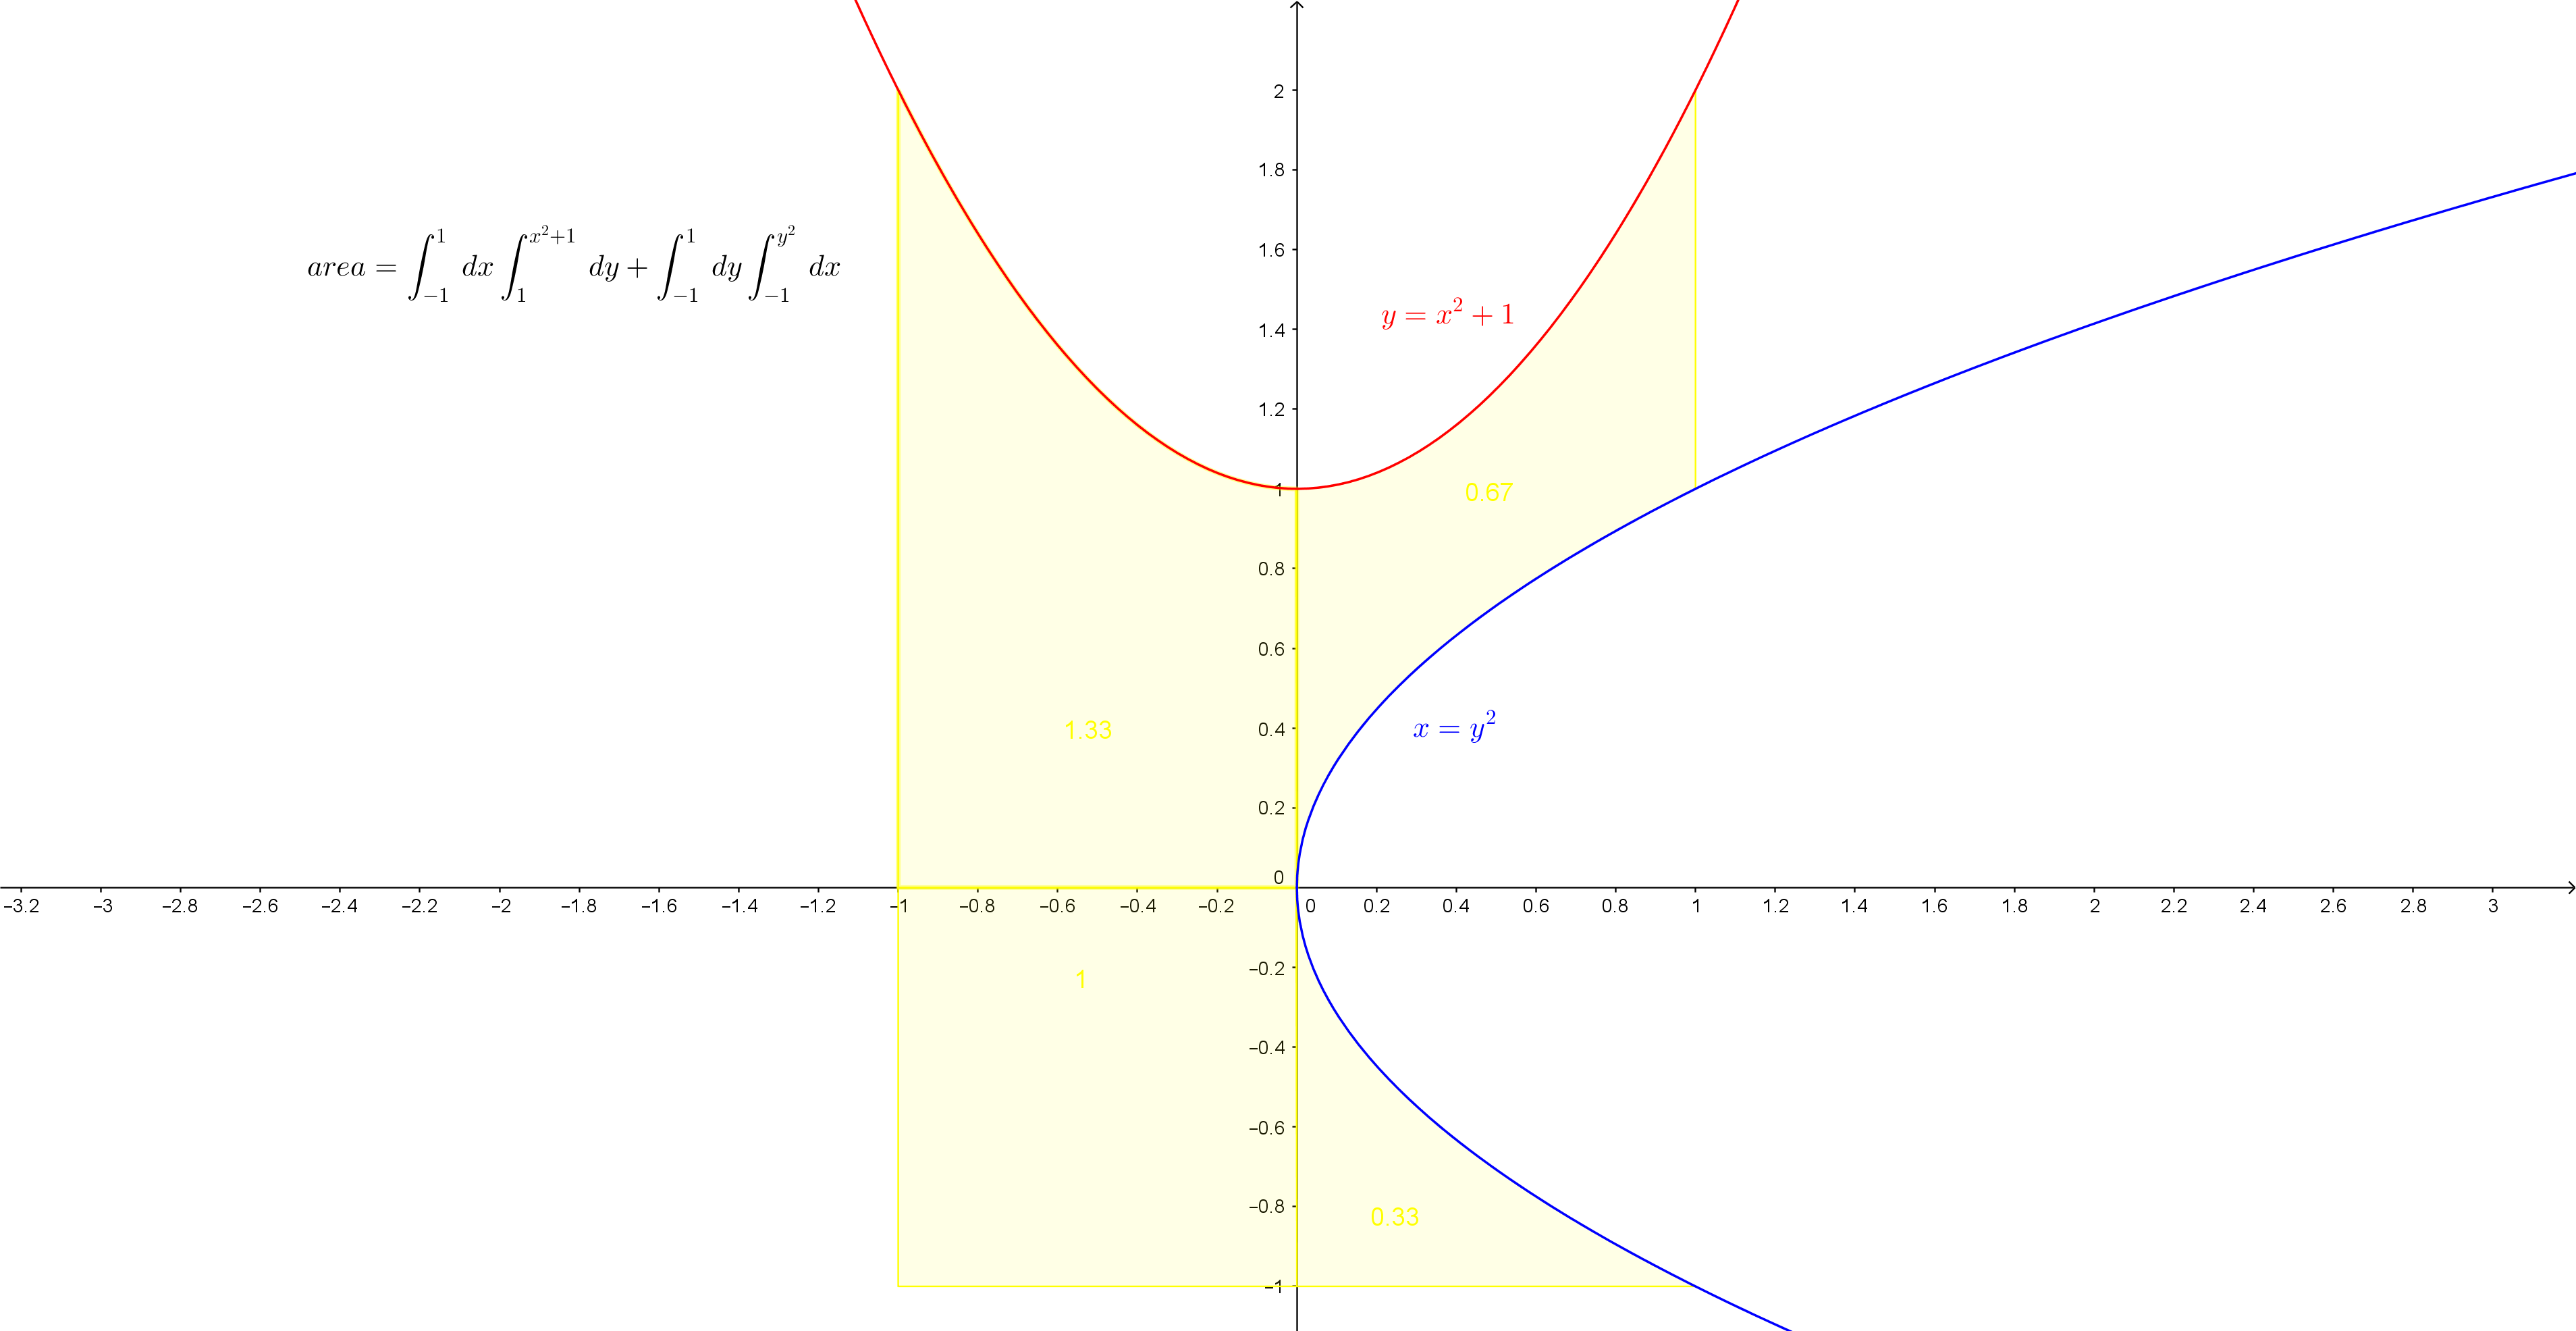
\includegraphics[width=0.5\textwidth]{v08_a08_e01.png}		
	\end{figure}
	
	\begin{align*}
		a = \int_{-1}^0 dx \int_0^{x^2 + 1} dy + \int_{-1}^0 dx \int_{-1}^0 dy + \int_0^{y^2} dx \int_{-1}^0 dy + \int_0^1 dx \int_{\sqrt{x}}^{x^2 + 1} =\\ \int_{-1}^0 dx\left(\int_0^{x^2 + 1} dy + \int_{-1}^0 dy\right)  + \int_0^{y^2} dx \int_{-1}^0 dy + \int_0^1 dx \int_{\sqrt{x}}^{x^2 + 1} =\\ \int_{-1}^0 dx \left([y]_0^{x^2 + 1} + [y]_{-1}^0\right)  + \int_{-1}^0 dy\, [x]_0^{y^2} + \int_0^1 dx\, [y]_{\sqrt{x}}^{x^2 + 1} =\\ \int_{-1}^0 dx\, \left(x^2 + 1 + 1\right) + \int_{-1}^0 dy\, y^2 + \int_0^1 dx\, \left(x^2 + 1 - \sqrt{x}\right) =\\ \int_{-1}^0 \left(x^2 + 2\right) dx + \int_{-1}^0 y^2\, dy + \int_0^1 \left(x^2 - x^{\frac{1}{2}} + 1\right) dx =\\ \left[\dfrac{x^3}{3} + 2x\right]_{-1}^0 + \left[\dfrac{y^3}{3}\right]_{-1}^0 + \left[\dfrac{x^3}{3} - \dfrac{x^{\frac{3}{2}}}{\left(\dfrac{3}{2}\right)} + x\right]_0^1 =\\ \left[\dfrac{x^3 + 6x}{3}\right]_{-1}^0 + \dfrac{1}{3}\left[y^3\right]_{-1}^0 + \left[\dfrac{x^3}{3} - \dfrac{2\sqrt{x^3}}{3} + x\right]_0^1 =\\ \dfrac{1}{3}\left[x\left(x^2 + 6\right)\right]_{-1}^0 + \dfrac{1}{3}\left[\overstrike{0^3} - (-1)^3\right] + \left[\dfrac{x^3 - 2\sqrt{x^3} + 3x}{3}\right]_0^1 =\\ \dfrac{1}{3}\left[\overstrike{0\left(0^2 + 6\right)} - (-1)\left((-1)^2 + 6\right)\right] + \dfrac{1}{3} + \dfrac{1}{3}\left[x^3 - 2\sqrt{x^3} + 3x\right]_0^1 =\\ \dfrac{7}{3} + \dfrac{1}{3} + \dfrac{1}{3}\left[1^3 - 2\sqrt{1^3} + 3\cdot1 \overstrike{- \left(0^3 - 2\sqrt{0^3} + 3\cdot0\right)}\right] = \dfrac{7}{3} + \dfrac{1}{3} + \dfrac{2}{3} =\\ \dfrac{7 + 1 + 2}{3} = \dfrac{10}{3} = 3,\overline{3}	
	\end{align*}	
	\begin{align*}
		a = \int_{-1}^1 dx \int_1^{x^2 + 1} dy + \int_{-1}^{y^2} dx \int_{-1}^1 dy = \int_{-1}^1 dx\, [y]_1^{x^2 + 1} + \int_{-1}^1 dy\, [x]_{-1}^{y^2} =\\ \int_{-1}^1 dx\, \left(x^2 \overstrike{+ 1 - 1}\right) + \int_{-1}^1 dy\, \left(y^2 + 1\right) = \left[\dfrac{x^3}{3}\right]_{-1}^1 + \left[\dfrac{y^3}{3} + y\right]_{-1}^1 =\\ \dfrac{1}{3}\left[x^3\right]_{-1}^1 + \dfrac{1}{3}\left[y\left(y^2 + 3\right)\right]_{-1}^1 =\\ \dfrac{1}{3}\left(\left[1^3 - (-1)^3\right] + \left[1\left(1^2 + 3\right) - (-1)\left((-1)^2 + 3\right)\right]\right)\dfrac{1}{3}(2 + 4 + 4) = \frac{10}{3} = 3,\overline{3}
	\end{align*}
\end{enumerate}